\documentclass[11pt,a4paper]{ltjsarticle}
% Compile with LuaLaTeX

% =========================
% Packages
% =========================
\usepackage{luatexja}
\usepackage{graphicx}
\usepackage{hyperref}
\usepackage{amsmath,amssymb,mathtools}
\usepackage{xcolor}
\usepackage{float}
\usepackage{subcaption}
\usepackage{booktabs}
\usepackage{enumitem}
\usepackage{geometry}
\usepackage{caption}

\geometry{margin=22mm}
\setcounter{tocdepth}{3}
\setlength{\parskip}{0.6mm}

% =========================
% Colour system (presentaion/slide_style_v3.md, sec. 3)
%   Science Blue  : the main scientific subject / structural headings
%   Deep Indigo   : exceptional or critical structure (used sparingly)
%   Mist Lavender : low-salience support field
%   Midnight Ink  : text, rules, neutral geometry (replaces pure black)
% Colour encodes argumentative role, not category.
% =========================
\definecolor{scienceblue}{HTML}{1C3177}
\definecolor{deepindigo}{HTML}{4B0082}
\definecolor{mistlavender}{HTML}{E8EAF1}
\definecolor{midnightink}{HTML}{101426}

\color{midnightink}
\hypersetup{colorlinks=true, linkcolor=scienceblue, urlcolor=scienceblue,
            citecolor=scienceblue}

% figures are evidence: neutral, restrained captions
\captionsetup{font=small, labelfont={bf,color=scienceblue},
              textfont={color=midnightink}, justification=justified}

% =========================
% User information
% =========================
\title{Weekly Report: Ultra-High-Pressure ODMR --- \\ Should we introduce a lock-in amplifier?}
\author{Risei Abe}
\date{Week: 2026/08/09 -- 2026/08/15}

% =========================
% Custom commands
% =========================
% Section heading: Science Blue label over a thin Midnight Ink rule.
\newcommand{\sectionblock}[1]{%
  \par\vspace{2.6mm}%
  \noindent{\large\bfseries\color{scienceblue}#1}\par\nobreak
  \vspace{0.4mm}%
  \noindent{\color{midnightink}\rule{\linewidth}{0.4pt}}\par\nobreak
  \vspace{-1.8mm}%
}

% Reserved for structure that has acquired special meaning in the argument.
\newcommand{\critical}[1]{\textcolor{deepindigo}{#1}}

\newcommand{\todo}[1]{\textcolor{deepindigo}{#1}}

\begin{document}

% title block in the deck palette
\makeatletter
\renewcommand{\maketitle}{%
  \begin{center}
    {\LARGE\bfseries\color{scienceblue}\@title\par}
    \vspace{2.5mm}
    {\normalsize\color{midnightink}\@author\par}
    \vspace{1mm}
    {\small\color{midnightink}\@date\par}
  \end{center}
  \vspace{1mm}
  {\color{scienceblue}\rule{\linewidth}{0.8pt}}
  \vspace{2mm}
}
\makeatother
\maketitle

% =========================================================
% 1. Question / Purpose
% =========================================================
\sectionblock{Question}

\begin{quote}
\colorbox{mistlavender}{\parbox{\dimexpr\linewidth-2\fboxsep}{%
A lock-in cannot beat shot noise, it can only move the measurement above the technical $1/f$ noise, so at what detector noise knee $f_{knee}$ does modulated detection actually start to improve the precision $\sigma_D$ of the fitted ODMR line centre, and which modulation scheme should we use?}}
\end{quote}

% =========================================================
% 2. Hypothesis
% =========================================================
\sectionblock{Hypothesis}

If the technical noise has relative PSD $S(f) = S_0(1 + f_{knee}/f)$ with $S_0$ pinned to the shot-noise floor, then a DC sweep --- which reads the line out at $\sim 1/T_{sweep} \sim 2$\,Hz --- should degrade as $\sqrt{f_{knee}}$ while modulated schemes stay flat, so there should be a break-even $f_{knee}$ below which plain DC averaging is better because modulation throws away duty cycle.

% =========================================================
% 3. Evidence / Interpretation
% =========================================================
\sectionblock{Evidence / Interpretation}

\begin{figure}[H]
  \centering
  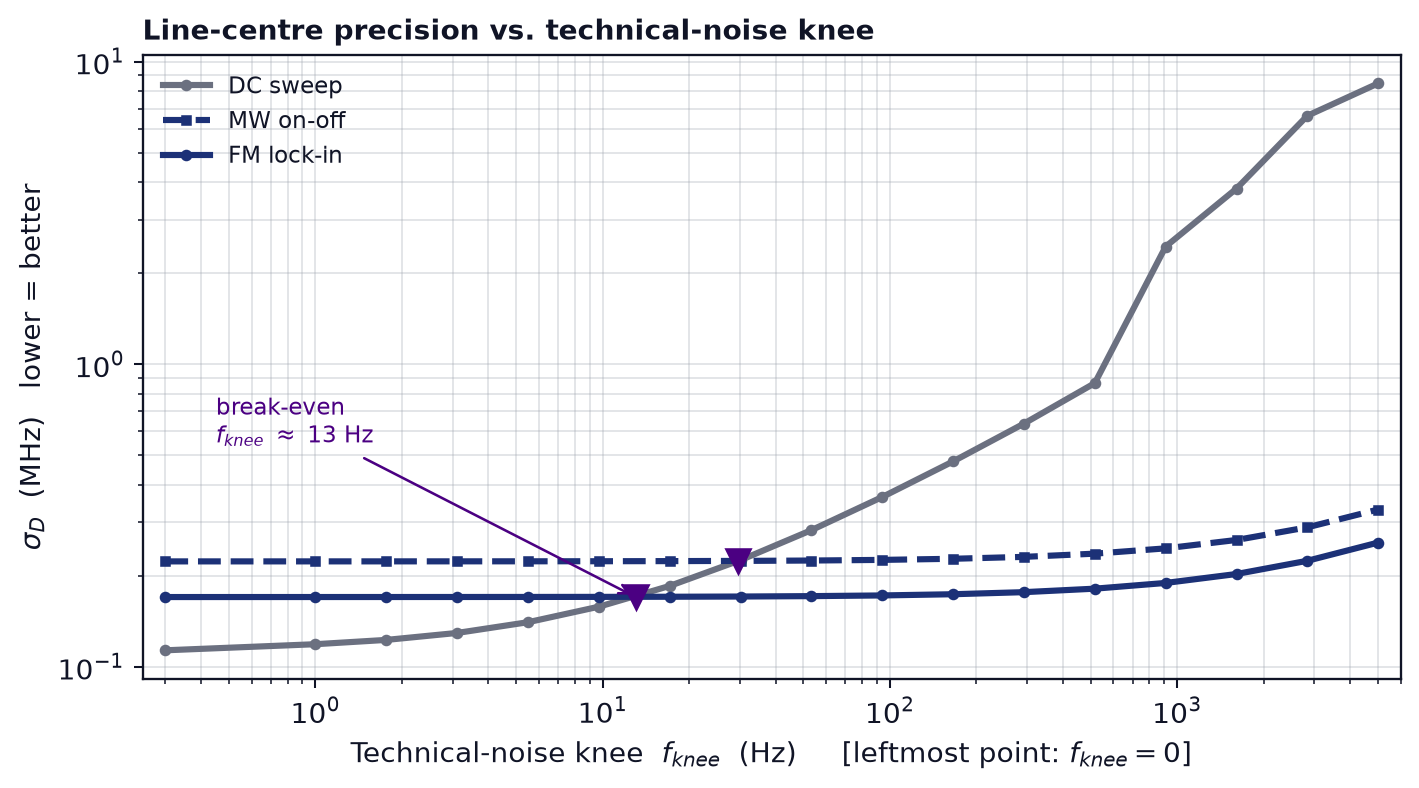
\includegraphics[width=0.88\linewidth]{image/lockin_decision_curve.png}
  \vspace{-1mm}
  \caption{Monte-Carlo $\sigma_D$ (200 realisations, identical total measurement time and identical noise realisation per trial) for a DC sweep, MW on-off chopping and FM lock-in, as a function of the technical-noise knee. Triangles mark the break-even knees.}
  \label{fig:lockin}
\end{figure}
\vspace{-3mm}

\begin{itemize}[leftmargin=8mm]
  \item The break-even is at $f_{knee} \approx 13$\,Hz for FM and $\approx 30$\,Hz for on-off chopping: below that, DC averaging is genuinely better (0.113 vs 0.170\,MHz at $f_{knee}=0$, the cost of the modulation duty cycle), and above it DC collapses while both modulated schemes stay flat to within 35\% out to 5\,kHz.
  \item At a realistic $f_{knee} = 1$\,kHz the gain is $13.7\times$ in $\sigma_D$, FM beats on-off by $\approx 1.3\times$ at its optimal dither depth of $0.5\,\Delta\nu$, and the gain saturates once $f_{mod}$ exceeds $f_{knee}$ --- so a few kHz of modulation is enough and nothing is gained by going faster.
\end{itemize}

% =========================================================
% 4.  Gap / Failure
% =========================================================
\sectionblock{Gap / Failure}

\begin{itemize}[leftmargin=8mm]
  \item The simulation assumes purely multiplicative intensity noise, so it misses additive drifts (background creep, detector dark-current wander) that modulation rejects even better --- the quoted gains are therefore a lower bound.
  \item Our own $f_{knee}$ is unmeasured, and since the whole decision turns on that single number the answer is currently a criterion rather than a recommendation.
\end{itemize}

% =========================================================
% 5. Next Step
% =========================================================
\sectionblock{Next Step}

Digitise a few seconds of the MW-off photodetector record and take its power spectral density to read off $f_{knee}$ directly, which both settles the decision and shows whether software demodulation of that same record already delivers the gain without buying hardware.

% =========================================================
% 9. References
% =========================================================
\sectionblock{References}

\begin{enumerate}[leftmargin=8mm]
  \item A.\ Dr\'eau \emph{et al.}, ``Avoiding power broadening in optically detected magnetic resonance of single NV defects,'' Phys.\ Rev.\ B \textbf{84}, 195204 (2011).
  \item J.\,F.\ Barry \emph{et al.}, ``Sensitivity optimization for NV-diamond magnetometry,'' Rev.\ Mod.\ Phys.\ \textbf{92}, 015004 (2020).
  \item Repository: \texttt{code/lockin\_sim.py}, \texttt{code/fig7\_lockin.py} (this analysis).
\end{enumerate}

\end{document}
